\chapter{Spark Shuffle分析}

前面讲解了map端和reduce端对Task的不同处理方式,连接它们的桥梁即为Shuffle模块,shuffle用于打通map任务的输出与reduce任务的输入,map任务计算的中间输出结果按照key值哈希后分配给某一个reduce任务。

shuffle过程数据的传输情况可能非常负责
\begin{enumerate}[\bfseries 1]
	\item 数据量大;
	\item 单个Executor内存不足以放下处理完的数据时需要进行磁盘读写;
	\item 数据传输过程中需要压缩和解压缩;
	\item 跨节点传输时需要通过网络;
\end{enumerate}

正因为这众多的因素,shuffle无疑是调优的重点,理解shuffle的版本历史有助于了解shuffle优化的思路。

Shuffle的类型是在SparkContext初始化时确定的,Spark1.6版本如程序\ref{inputPrg:shuffleManager}所示
\begin{codeInput}{Scala}{ShuffleManager的初始化}{shuffleManager}
 //   指定shuffle的类型
 val shortShuffleMgrNames = Map(
 "hash" -> "org.apache.spark.shuffle.hash.HashShuffleManager",
 "sort" -> "org.apache.spark.shuffle.sort.SortShuffleManager",
 "tungsten-sort" -> "org.apache.spark.shuffle.sort.SortShuffleManager")
 val shuffleMgrName = conf.get("spark.shuffle.manager", "sort")
 val shuffleMgrClass = shortShuffleMgrNames.getOrElse(shuffleMgrName.toLowerCase, shuffleMgrName)
 val shuffleManager = instantiateClass[ShuffleManager](shuffleMgrClass)
\end{codeInput}

可以看出ShuffleManager默认类型为SortShuffleManager。

在Executor上执行ShuffleMapTask时,最终会调用ShuffleMapTask.runTask。核心逻辑如程序\ref{inputPrg:runTaskGetShuffleManager}所示
\begin{codeInput}{Scala}{ShuffleMapTask获取ShuffleWriter}{runTaskGetShuffleManager}
 //从SparkEnv中获取shuffleManager
 val manager = SparkEnv.get.shuffleManager
 //从manager中获取Writer,这里是SortShuffleWriter
 writer = manager.getWriter[Any, Any](dep.shuffleHandle, partitionId, context)
 //调用RDD开始运算,运算结果通过Writer进行持久化,之后将文件所有记录写入并创建索引文件,通过MapStatus告知下游Task
 writer.write(rdd.iterator(partition, context).asInstanceOf[Iterator[_ <: Product2[Any, Any]]])
 writer.stop(success = true).get
\end{codeInput}
\section{Shuffle Writer历史版本}
\subsection{Hash Based Shuffle Write}
在Spark1.0以前,由于不要求数据有序,shuffle write 的任务很简单:将数据 partition 好,并持久化。之所以要持久化,一方面是要减少内存存储空间压力,另一方面也是为了 fault-tolerance。

shuffle write 的任务很简单,那么实现也很简单:将 shuffle write 的处理逻辑加入到 ShuffleMapStage(ShuffleMapTask 所在的 stage) 的最后,该 stage 的 final RDD 每输出一个 record 就将其 partition 并持久化。此种类型的Writer工作方式如图\ref{fig:hashShuffleWriter}所示, 从图中可以看出4 个 ShuffleMapTask 要在同一个 worker node 上运行,CPU core 数为 2,可以同时运行两个 task。每个 task 的执行结果(该 stage 的 finalRDD 中某个 partition 包含的 records)被逐一写到本地磁盘上。每个 task 包含 R 个缓冲区,R = reducer 个数(也就是下一个 stage 中 task 的个数),缓冲区被称为 bucket\footnote{其实 bucket 是一个广义的概念,代表 ShuffleMapTask 输出结果经过 partition后要存放的地方,这里为了细化数据存放位置和数据名称,仅仅用 bucket 表示缓冲区。},其大小为spark.shuffle.file.buffer.kb ,默认是 32KB(Spark 1.1 版本以前是 100KB)。
\begin{figure}[H] 
	\centering
	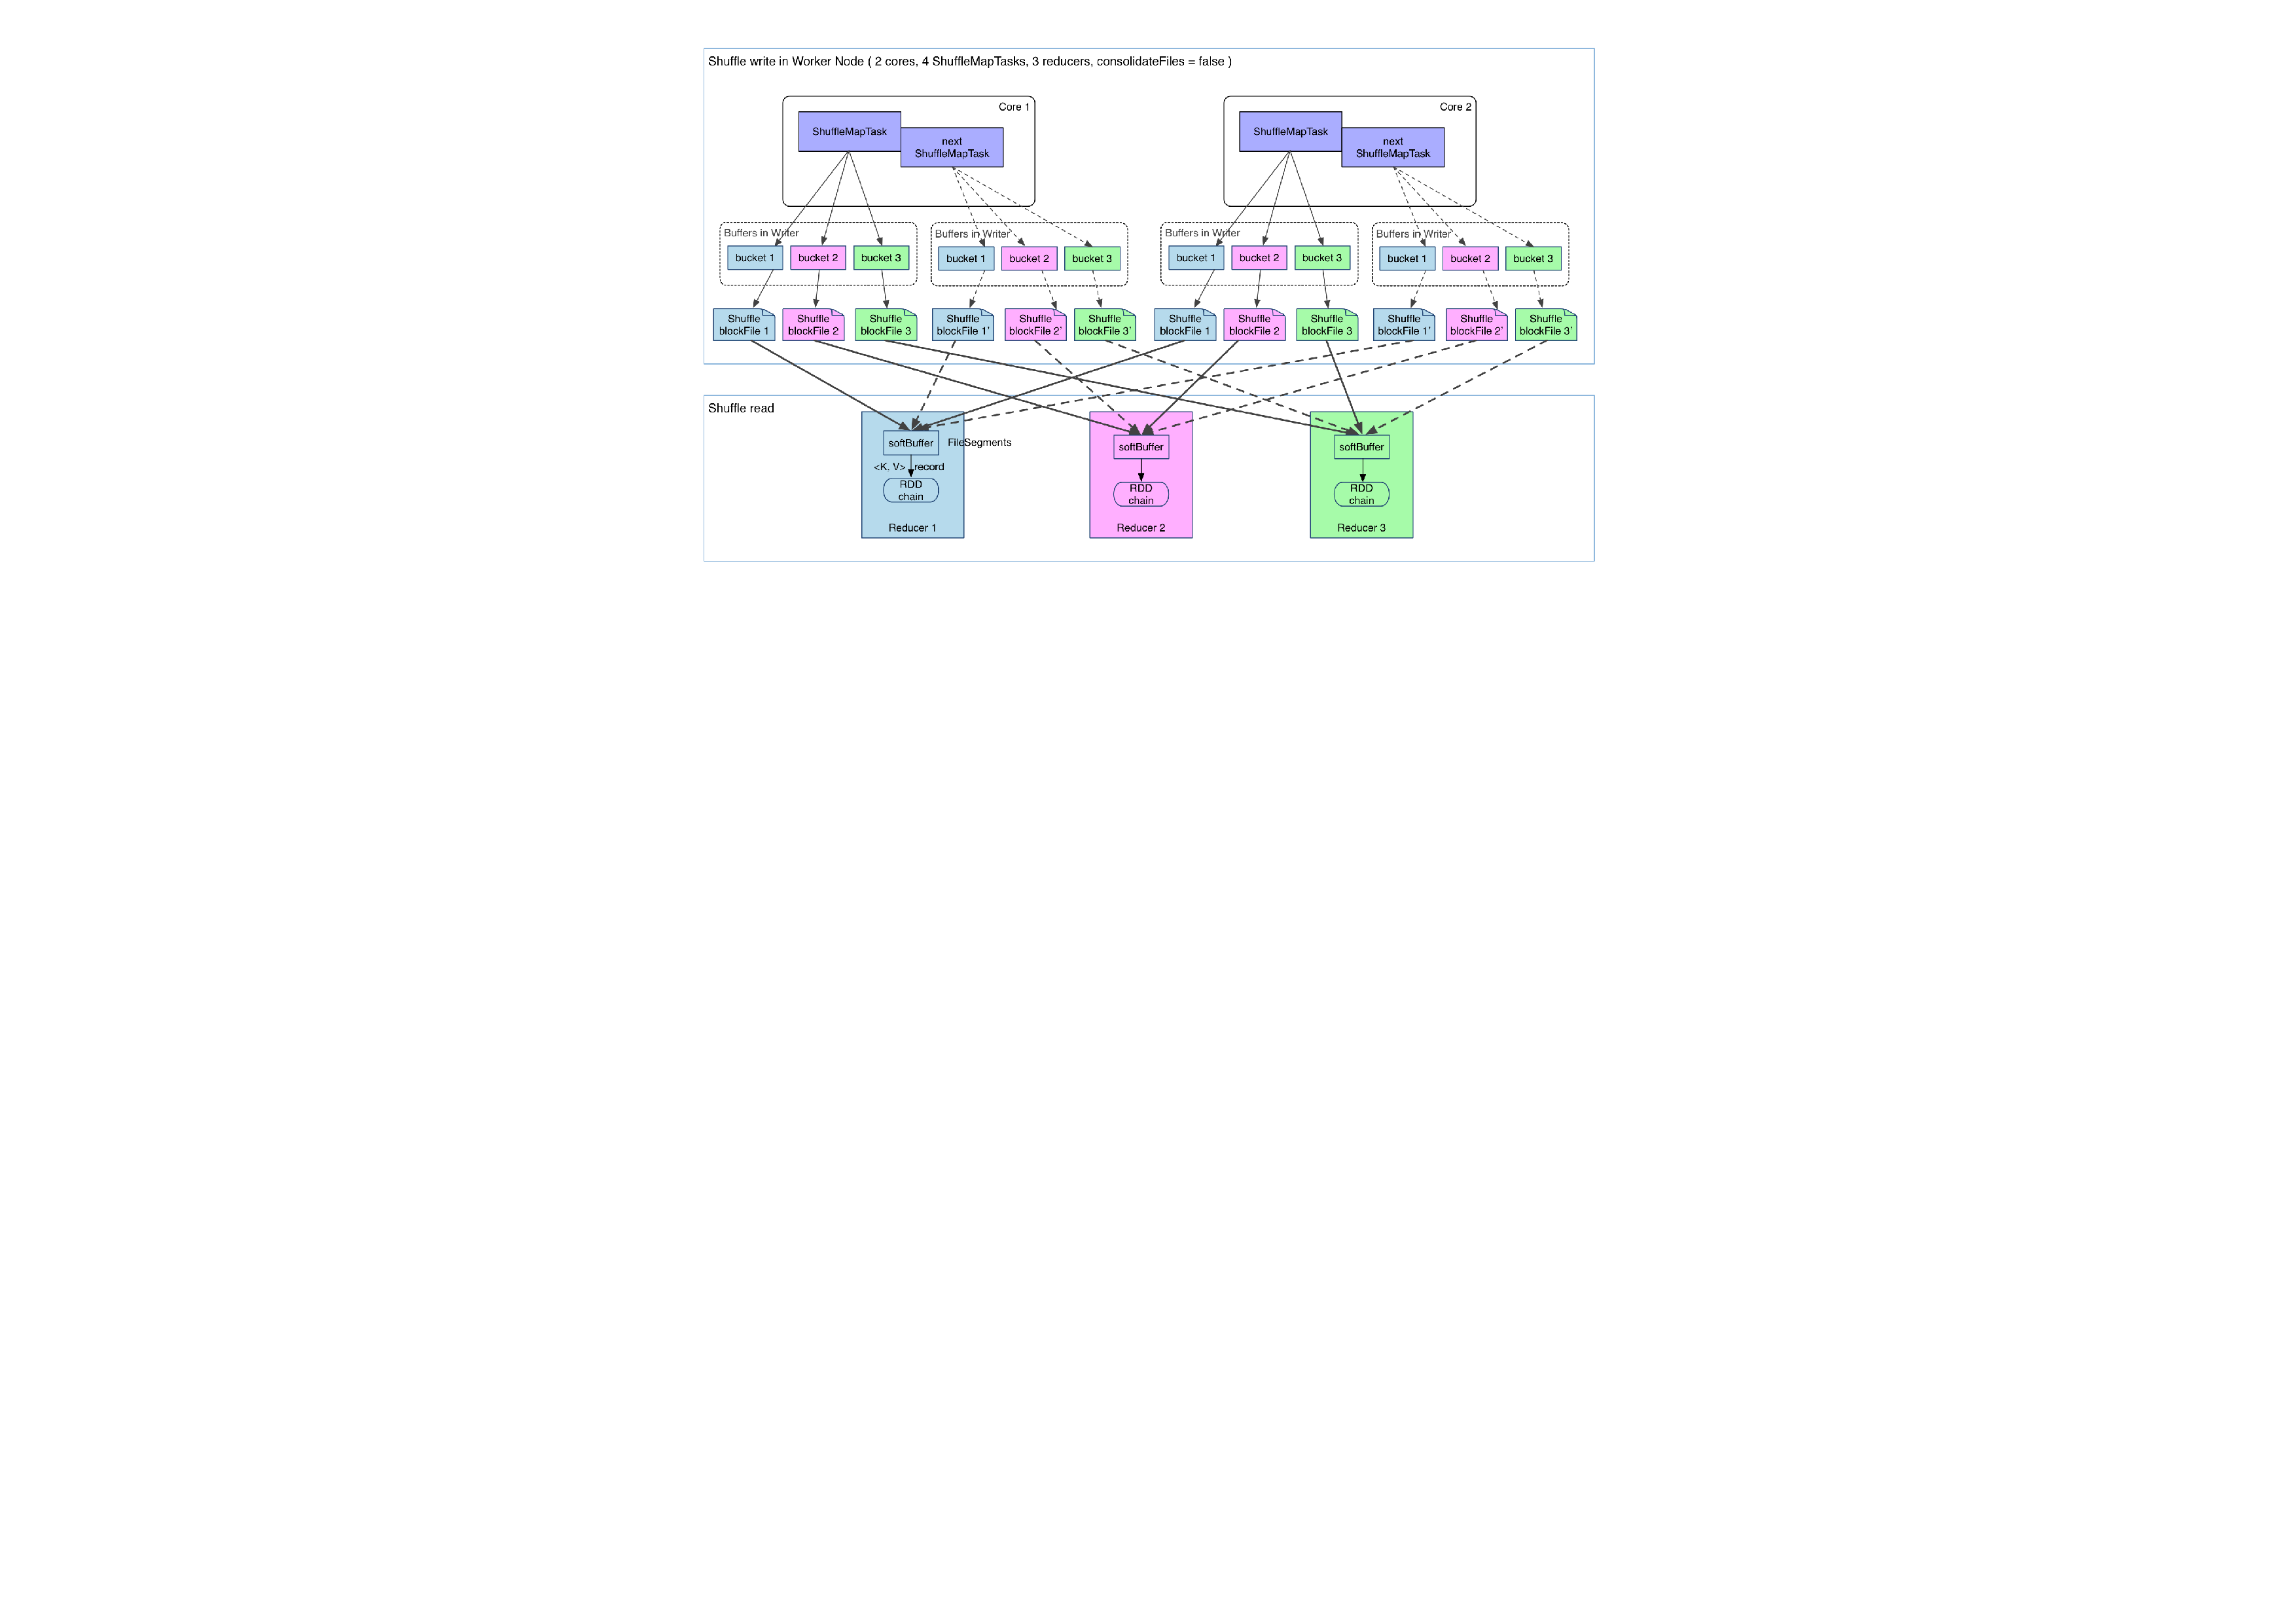
\includegraphics[width=\textwidth]{figures/hashShuffleWriter.pdf}
	\caption{早期的ShuffleWriter工作原理}
	\label{fig:hashShuffleWriter}
\end{figure}
\subsection{Hash Based Shuffle Write存在的问题}

由于ShuffleMapTask需要为每个下游的Task创建一个单独的文件,因此文件的数量就是M*R\footnote{M为shuffleMapTask的数量,R为reduce端Task的数量}个。如果单机28个cpu core,假设节点上20个core用于ShuffleMapTask,R数量为1000个,那么逻辑上会有20000个文件。在实际运行中,Task的数量会更多,这种ShuffleWriter的实现会带来一下问题:
\begin{enumerate}[\bfseries 1]
	\item 缓冲区占用内存空间大
	
	每个节点都可能同时打开多个文件,每次打开文件都会占用一定内存。如上面的20000个文件,每个writer Handler默认需要100KB内存,单个节点就可能达到2GB的内存,当Map端和Reduce同时增加10倍时,整体的内存会更吓人。
	\item 系统随机读增多
	
	当系统存在很多文件比较小但数量比较多的时候,而且机械硬盘在随机读方面的性能特别差,非常容易出现性能瓶颈。
\end{enumerate}
\subsection{Shuffle Consolidate Writer}

为了解决上一小节中Shuffle产生文件较多的问题,之后的Shuffle加入了Consolidate Files机制,它的目标就是减少Shuffle过程文件产生过多的问题,当然第一个问题还是没有解决。它的思想是针对同一个核运行多个ShuffleMapTask的情况下,众多的ShuffleMapTask会将记录写到同一个文件中,下一个会以追加的方式写入而不是新建文件。这样文件数就变为core\footnote{这里指核的数量}*R个文件。此种模式下运行原理如图\ref{fig:consolidate}所示
\begin{figure}[H] 
	\centering
	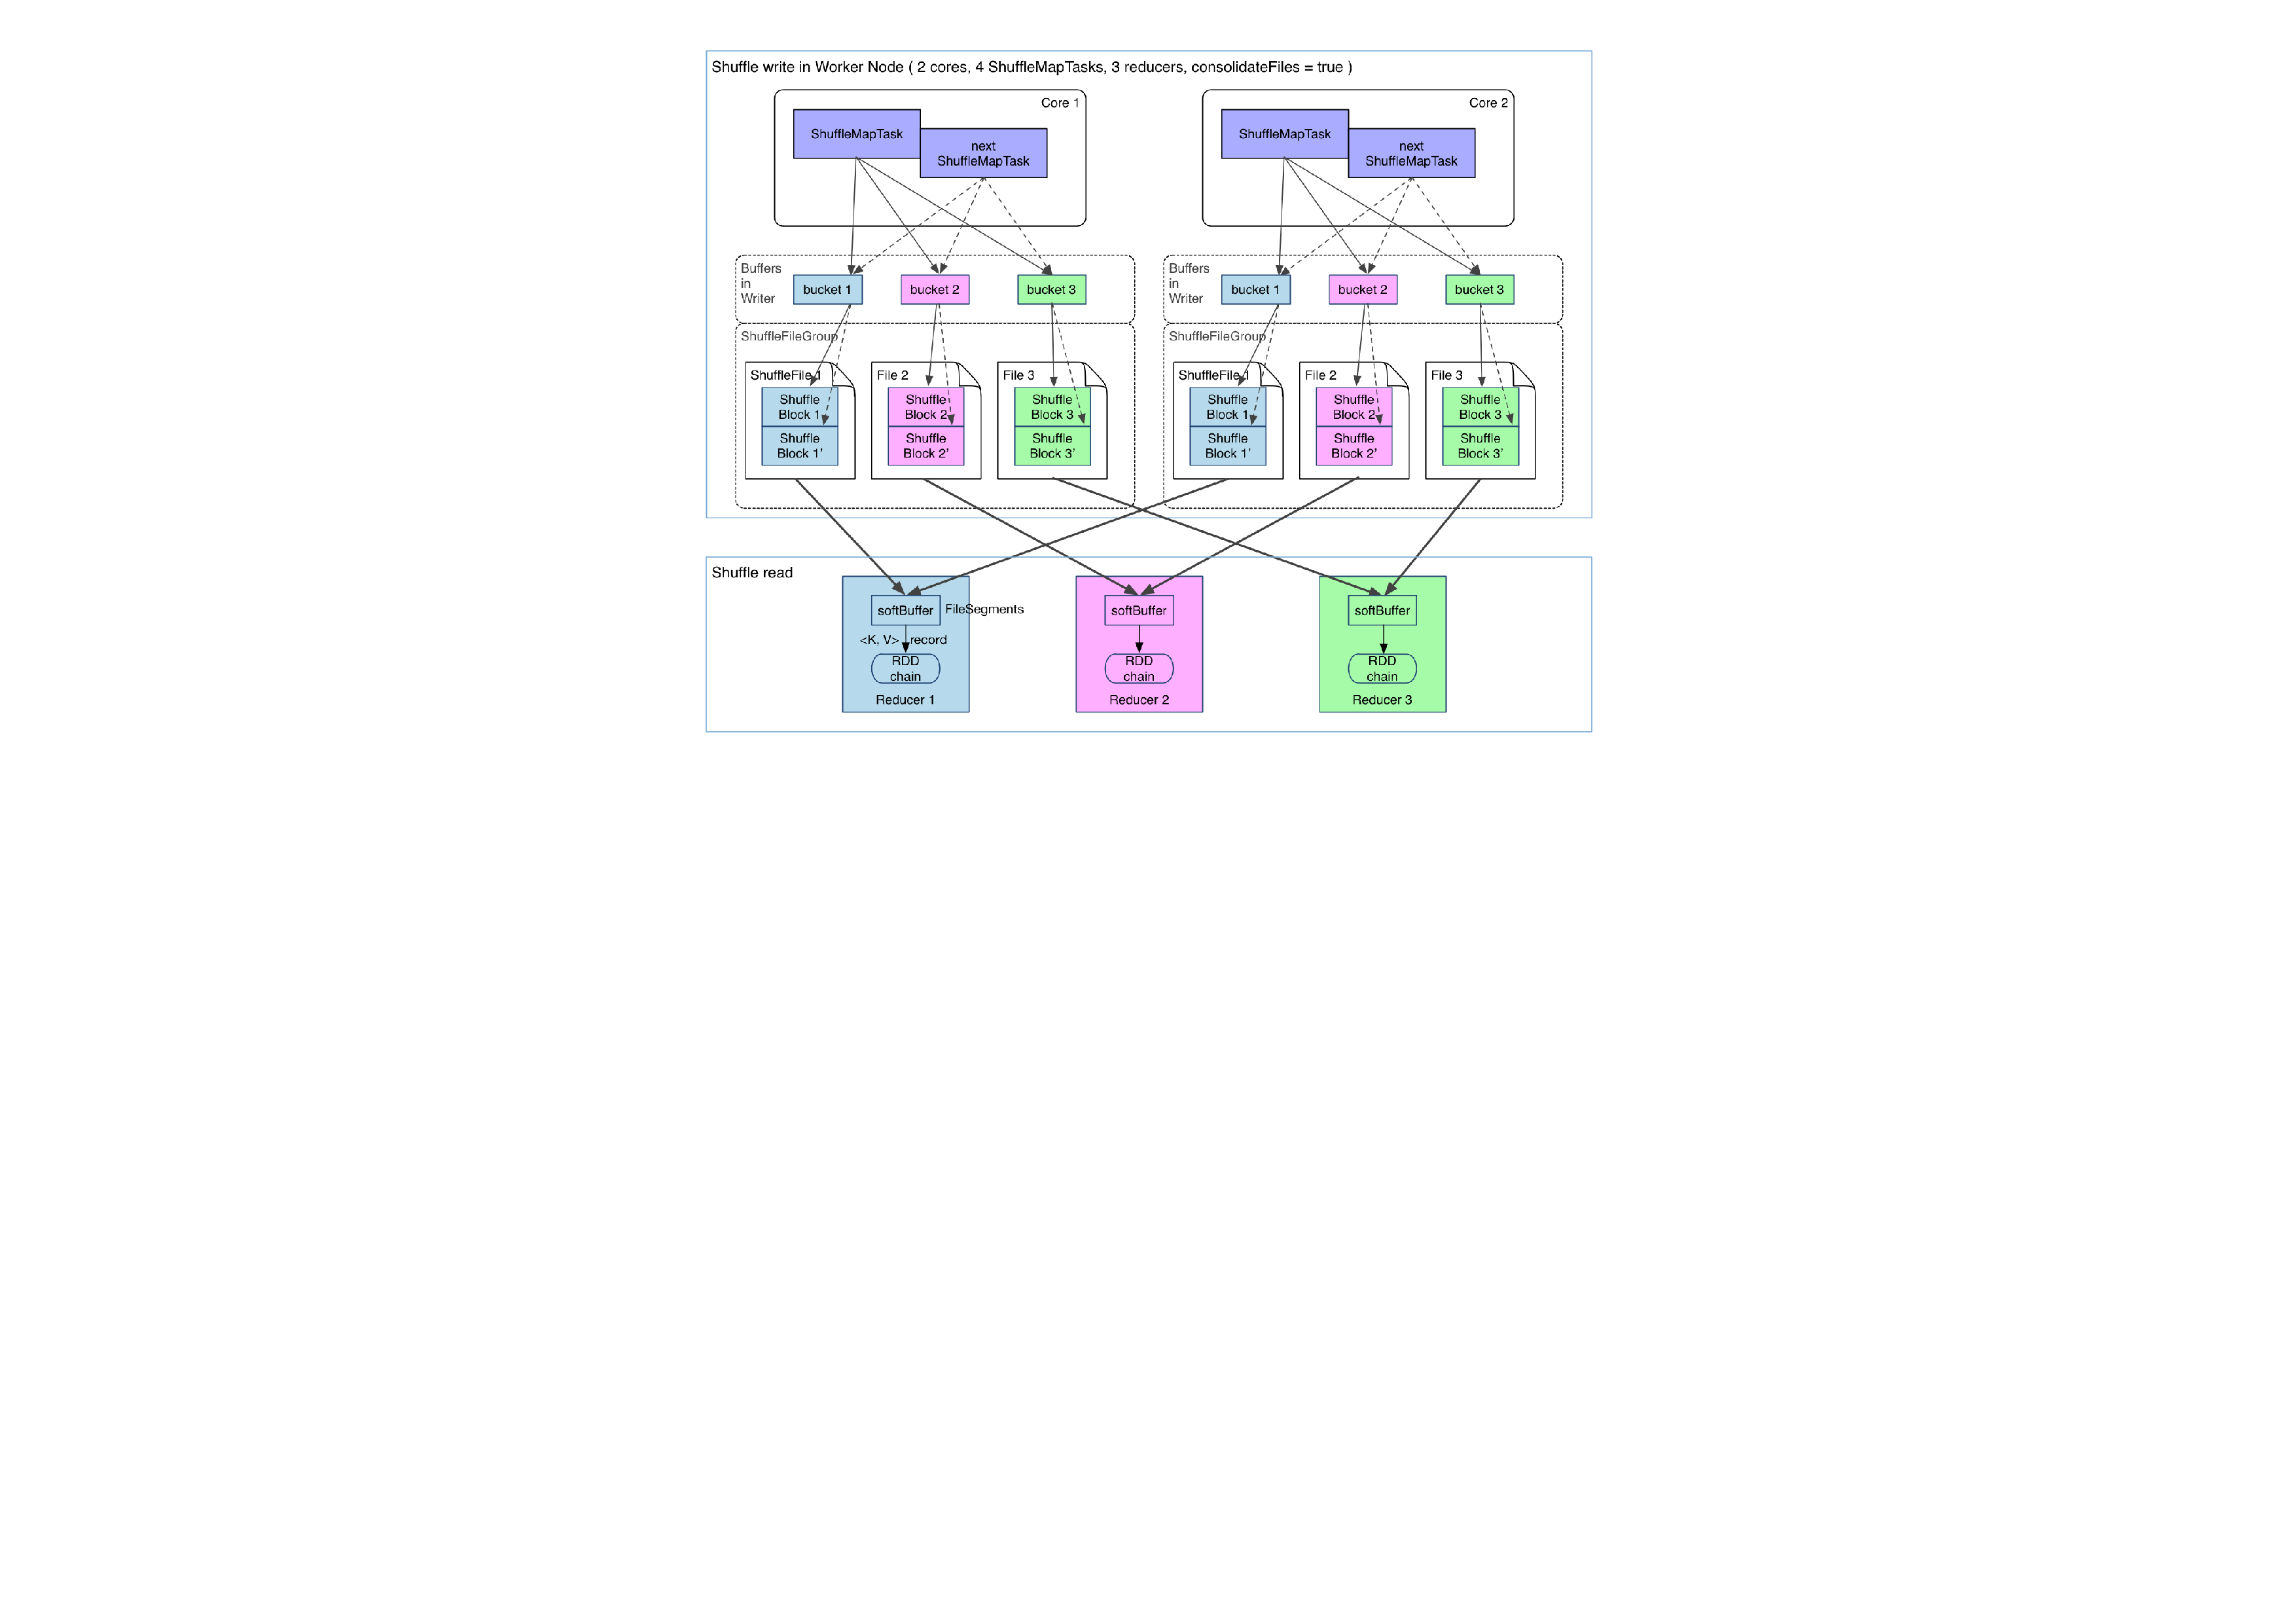
\includegraphics[width=\textwidth]{figures/consolidate.pdf}
	\caption{Shuffle Consolidate Files工作原理}
	\label{fig:consolidate}
\end{figure}

不过这种模式下当每个core只运行一个ShuffleMapTask时,那么就和原来的机制一样了。但是当ShuffleMapTask明显多于core数量时,这种模式下可以显著减少文件的数量。这里还剩下一个问题,下游的Task如何区分文件的不同部分?这部分在后面小节中讲述。

针对Shuffle Consolidate遗留的问题,Spark重新建立了一套Shuffle机制。也就是下面讲述的SortShuffle,这个已经是当前Spark版本的默认选项。
\subsection{Sort Based Write}
此方法的选择是在org.apache.spark.SparkEnv下完成的,本章开头部分已经说明。首先,每个ShuffleMapTask不会为每个Reducer生成一个单独的文件相反,它会将所有的结果写到一个文件里,同时生成一个Index文件,Reducer可以通过这个Index文件取得它需要处理的数据,减少了文件的数量。

Shuffle Map Task 会按照 key 相对应的 partition id 进行排序,对于属于同一个 partition 的 keys 可选的进行或不进行排序。因为对于不需要排序的操作来说,这个排序是有损性能的。对于那些需要 Sort 的操作,比如 sortByKey,这个排序是由 Reducer 完成的。Sort Base Shuffle原理如图\ref{fig:sortshuffle}所示
\begin{figure}[H] 
	\centering
	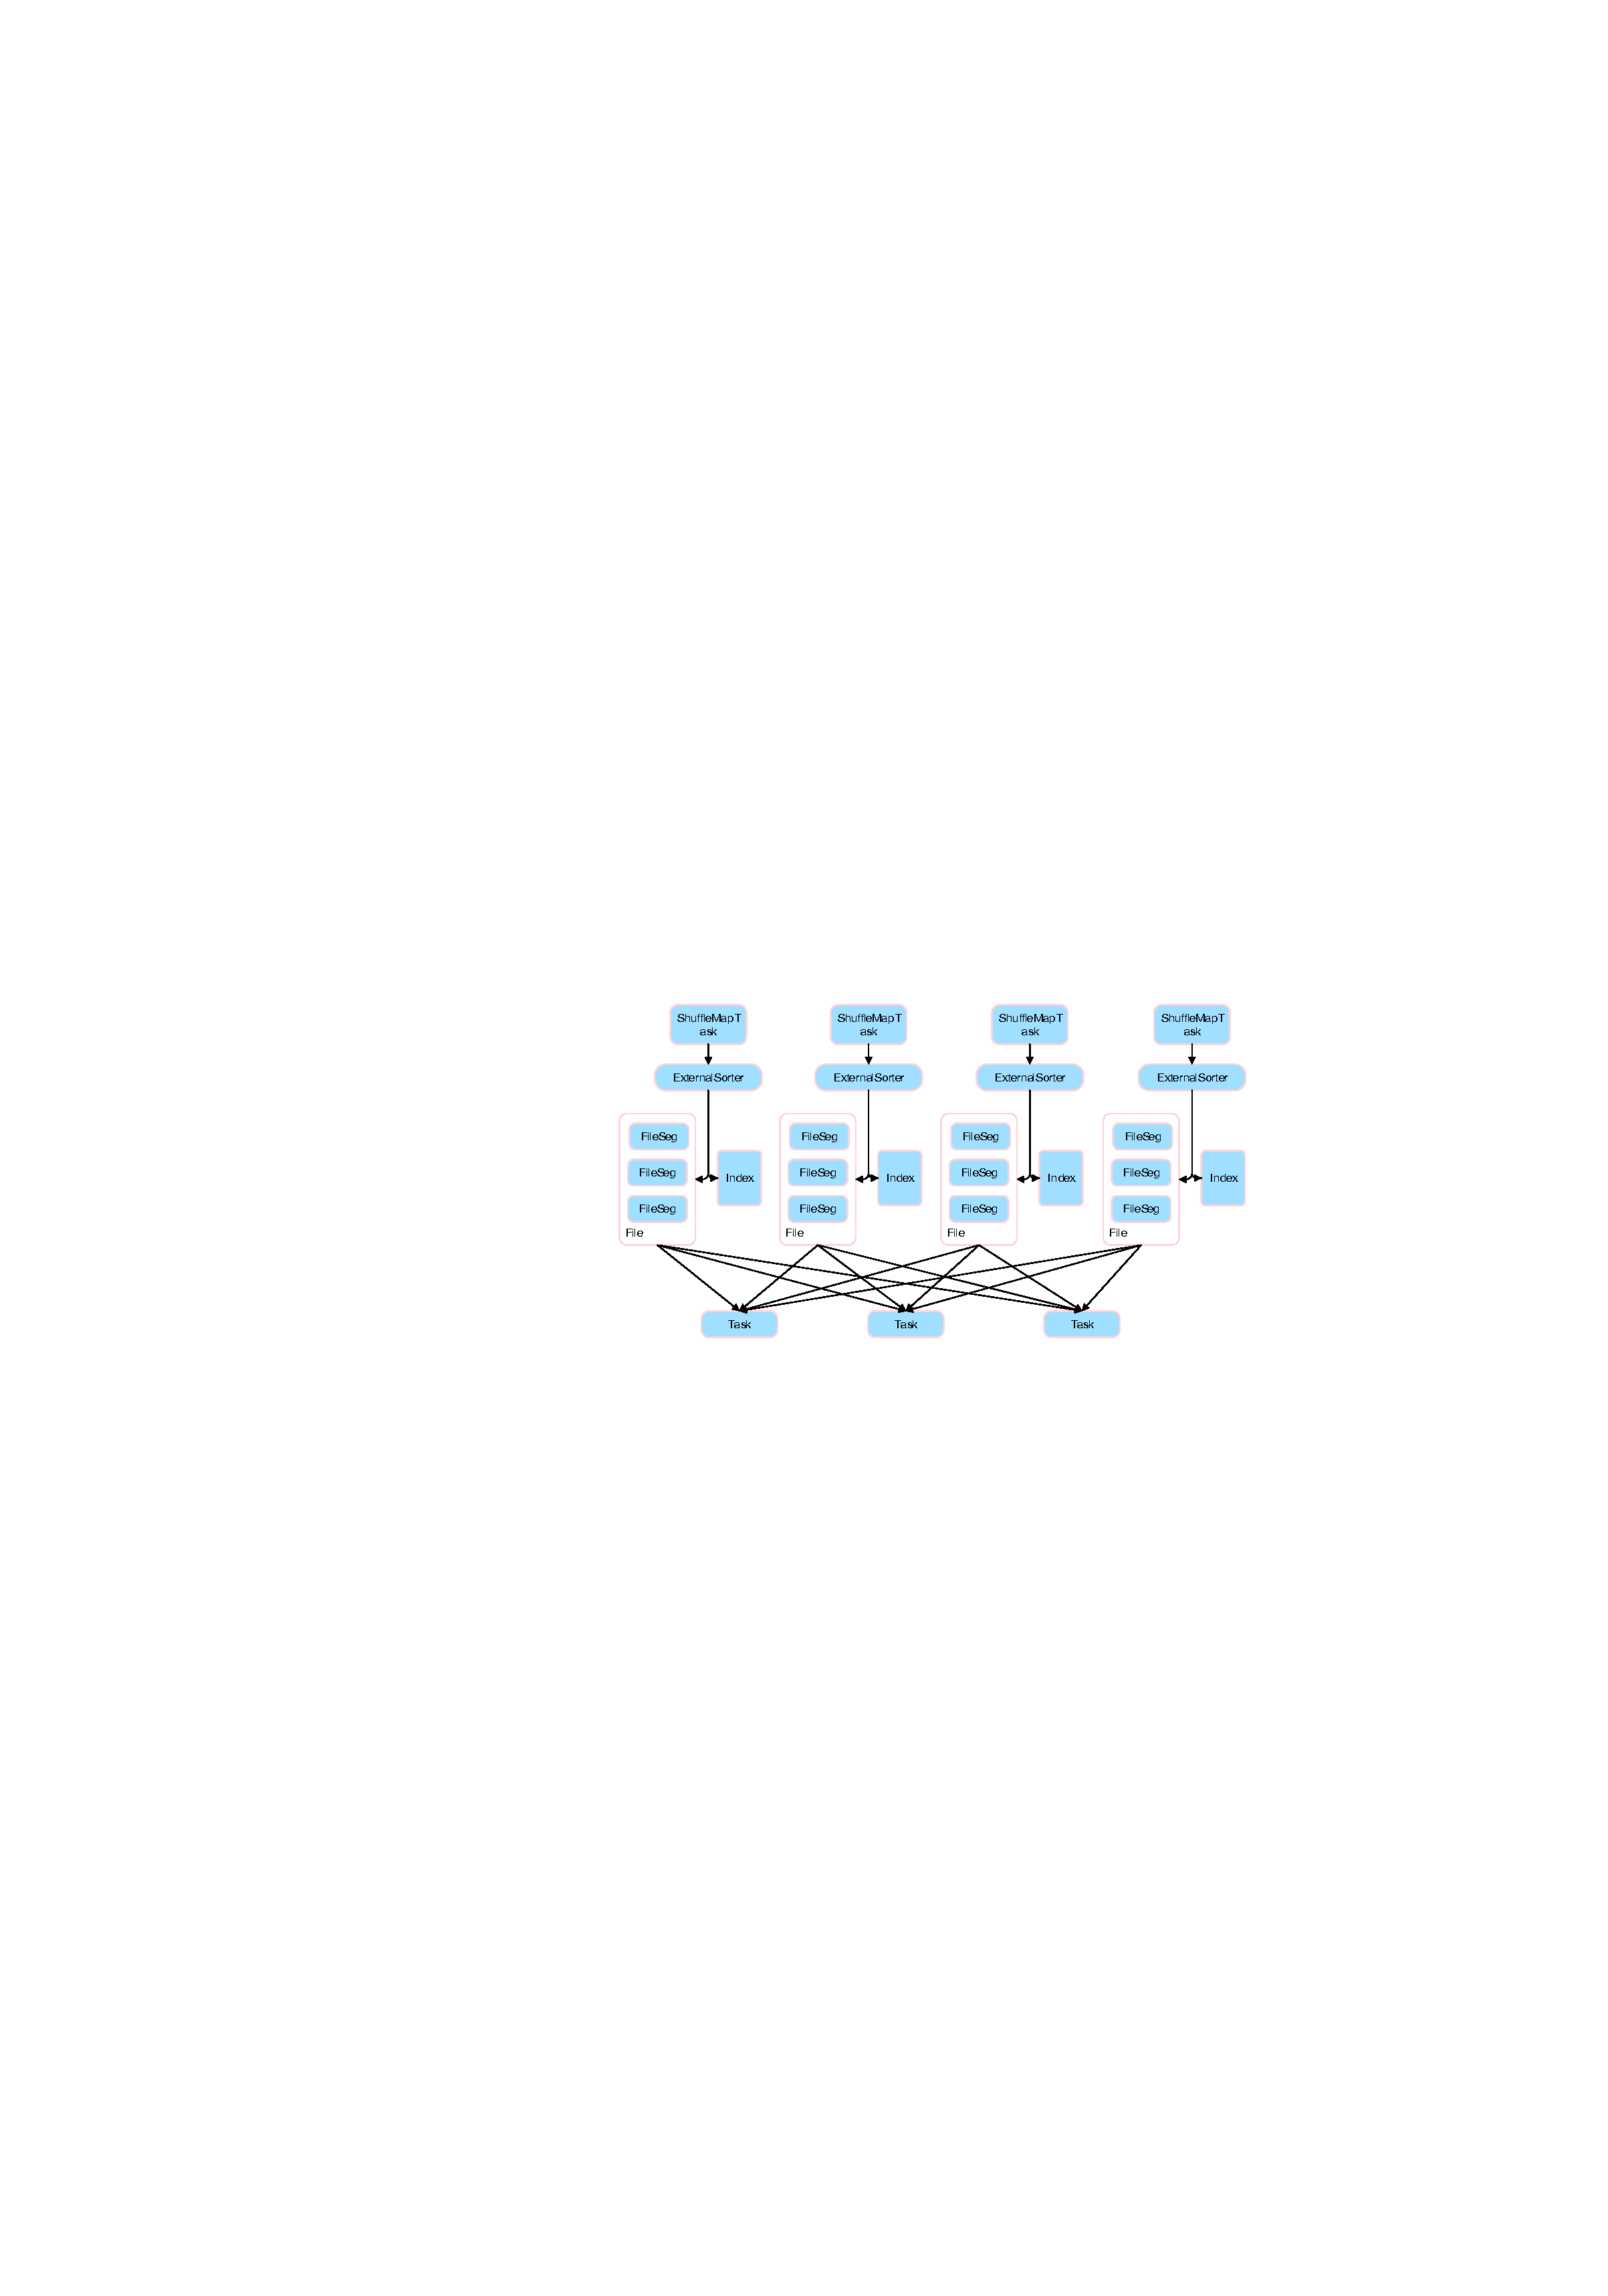
\includegraphics[width=\textwidth]{figures/sortshuffle.pdf}
	\caption{Sort Base Shuffle工作原理}
	\label{fig:sortshuffle}
\end{figure}

为了下游Task获取到其所需要的分区,生成文件的同时会附加Index文件,来记录不同分区的位置信息。
\section{Spark1.6版本Shuffle Write}
本节分析Spakr1.6中默认采用的SortShuffleManager对应的writer。SortShuffleManager中的getWriter会根据不同的ShuffleHandle产生相应的ShuffleWriter
\begin{enumerate}[\bfseries 1]
	\item SerializedShuffleHandle 对应 UnsafeShuffleWriter
	\item BypassMergeSortShuffleHandle 对应 BypassMergeSortShuffleWriter
	\item BaseShuffleHandle 对应 SortShuffleWriter
\end{enumerate}
\subsection{BaseShuffleHandle 对应 SortShuffleWriter}
其writer方法如程序\ref{inputPrg:sortShuffleWriter}所示
\begin{codeInput}{Scala}{SortShuffleWriter write方法实现}{sortShuffleWriter}
override def write(records: Iterator[Product2[K, V]]): Unit = {
  //如果数据需要在map端combine,则需要传入dep.aggregator,下面的这个dep.keyOrdering是空值,
  // 因为在spark的sortedshuffle中,数据是不排序的。这里的这个partitioner是用来为后续RDD构造partitions的
  sorter = if (dep.mapSideCombine) {
    require(dep.aggregator.isDefined, "Map-side combine without Aggregator specified!")
    new ExternalSorter[K, V, C](
    context, dep.aggregator, Some(dep.partitioner), dep.keyOrdering, dep.serializer)
  } else {
    //如果数据不需要在map端combine,则aggregator传None就行
    new ExternalSorter[K, V, V](context, aggregator = None, Some(dep.partitioner), ordering = None,dep.serializer)
  }
  //将数据先放入缓存中,如果缓存不够用spill到磁盘,在这一步也会对相同key值的数据进行combine操作
  sorter.insertAll(records)
  //打开一个文件
  val output = shuffleBlockResolver.getDataFile(dep.shuffleId, mapId)
  val tmp = Utils.tempFileWith(output)
  //构造blockId
  val blockId = ShuffleBlockId(dep.shuffleId, mapId, IndexShuffleBlockResolver.NOOP_REDUCE_ID)
  //将数据写入data文件
  val partitionLengths = sorter.writePartitionedFile(blockId, tmp)
  //将数据写入index文件
  shuffleBlockResolver.writeIndexFileAndCommit(dep.shuffleId, mapId, partitionLengths, tmp)
  //进行shuffle read时的一些参考信息
  mapStatus = MapStatus(blockManager.shuffleServerId, partitionLengths)
}
\end{codeInput}
程序\ref{inputPrg:sortShuffleWriter}中的ExternalSorter有下面三个作用
\begin{enumerate}
	\item 实例化ExternalSorter
	\item 调用insertAll()方法对记录集进行操作
	\item 返回已经排序或者聚合之后的记录的迭代器
\end{enumerate}
\subsection{实例化ExternalSorter}
首先就是实例化ExternalSorter,这里有一个判断,如果要进行map端的combine操作的话就需要指定Aggregator和Ordering,否则这两个参数为None。本例采用的reduceByKey就进行了Map端的combine操作,由ReduceByKey算子构造ShuffleRDD的过程如图\ref{fig:instantiateExternalSorter}所示
\begin{figure}[H] 
	\centering
	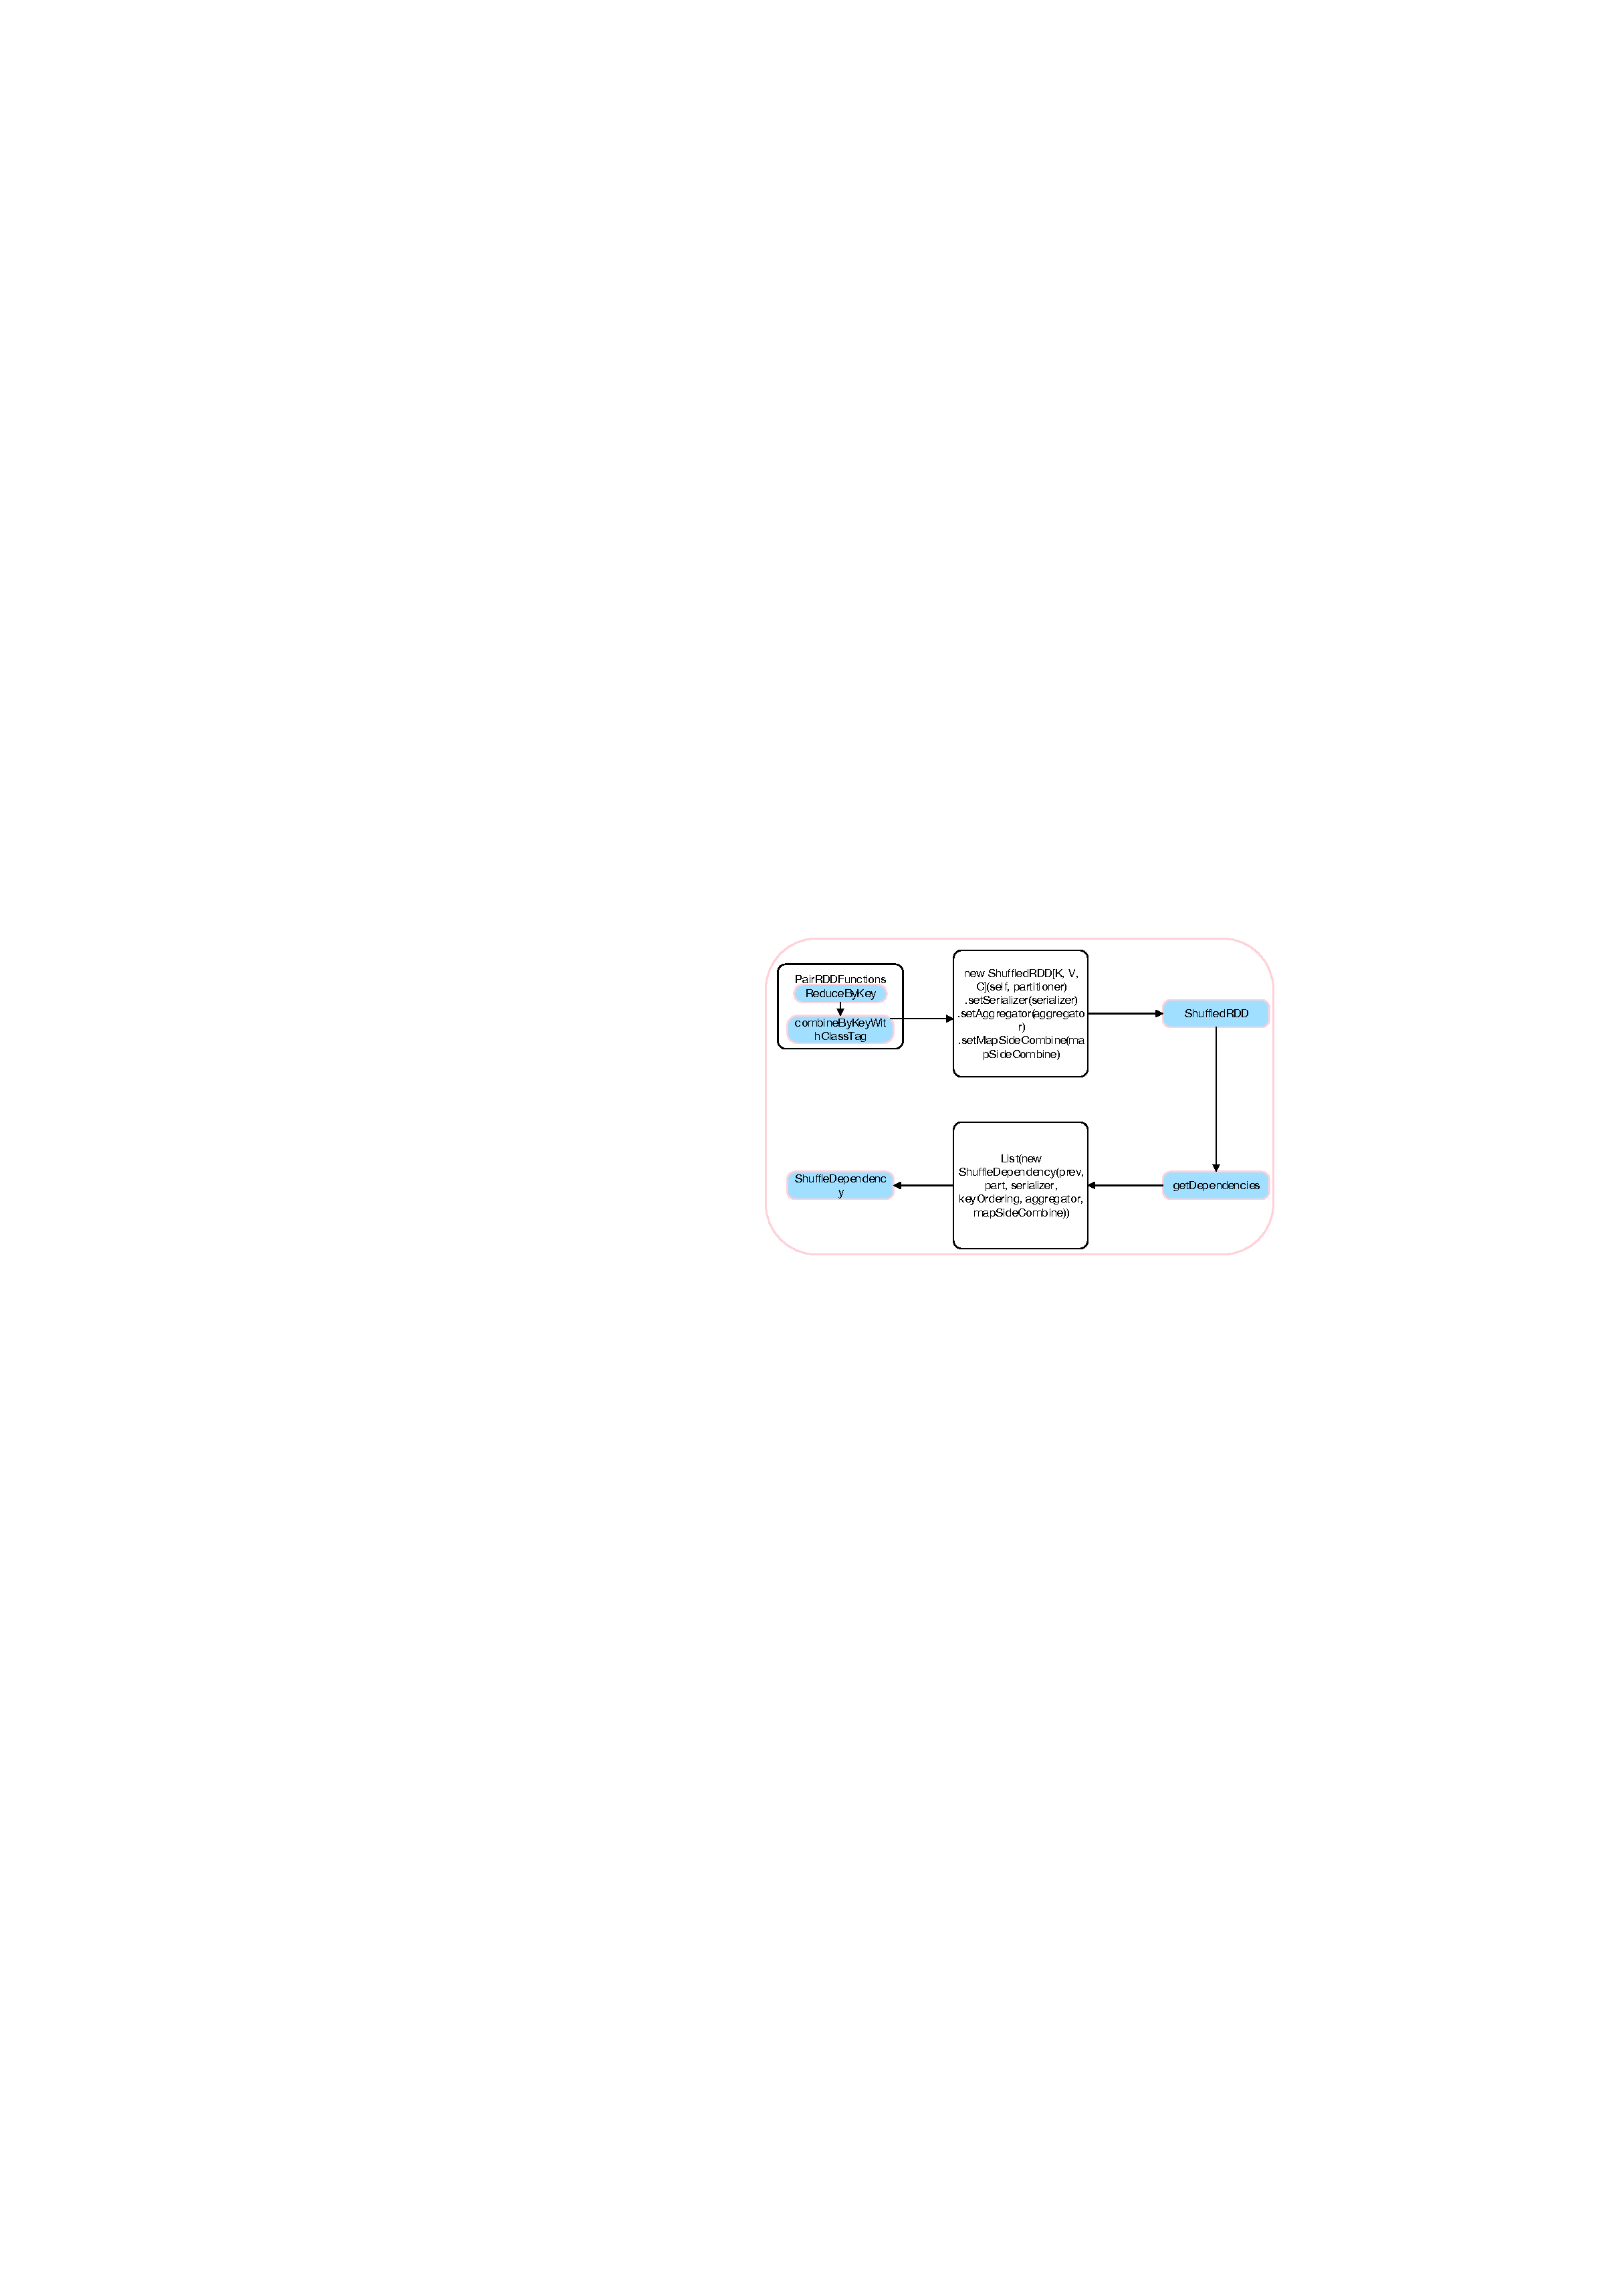
\includegraphics[width=\textwidth]{figures/ReduceByKey.pdf}
	\caption{ReduceByKey算子}
	\label{fig:instantiateExternalSorter}
\end{figure}
\subsection{shuffle写操作}
通过判断是否进行Map端combine操作而实例化出不同的ExternalSorter后,就会调用insertAll方法,将输入的记录写入到内存中,如果内存不足就spill到磁盘中,具体的实现我们来看insertAll方法,如程序\ref{inputPrg:insertAll}所示
\begin{codeInput}{Scala}{SortShuffleWriter insertAll方法实现}{insertAll}
def insertAll(records: Iterator[Product2[K, V]]): Unit = {
  val shouldCombine = aggregator.isDefined	
  //首先判断是否需要进行Map端的combine操作
  if (shouldCombine) {
    //如果需要进行Map端combine操作,使用PartitionedAppendOnlyMap作为缓存
    // mergeValue其实就是我们用reduceByKey的时候参数值,即_+_
    val mergeValue = aggregator.get.mergeValue
    //(C, V) => C  =>func
    //createCombiner其实是和mergeValue一样的,都是_+_,但是在使用createCombiner中只传了一个参数,所以另一个参///数默认采用默认值,这里为0
    val createCombiner = aggregator.get.createCombiner//V => C
    var kv: Product2[K, V] = null
    // 这个update也是一个函数,逻辑为如果某个Key已经存在记录record就使用上面获取的聚合函数进行聚合操作,
    // 如果不存在记录,就使用createCombiner方法进行初始化操作
    val update = (hadValue: Boolean, oldValue: C) => {
      if (hadValue) mergeValue(oldValue, kv._2) else createCombiner(kv._2)
    }
    //遍历所有的records
    while (records.hasNext) {
      //记录spill的频率,每当read一条record的时候就会记录一次
      addElementsRead()
      //使用kv存储当前读的records
      kv = records.next()
      //对key相同的记录的value进行合并
      //更新map中的数据,其中private var map = new PartitionedAppendOnlyMap[K, C],
      // 如果需要进行combine就将数据放在map中,然后在map中对数据进行更新操作
      map.changeValue((getPartition(kv._1), kv._1), update)
      //判断是否需要进行spill操作
      maybeSpillCollection(usingMap = true)
    }
  } else {
    // 如果不需要进行Map端的聚合操作,就直接将记录放到buffer(PartitionedPairBuffer)中
    while (records.hasNext) {
      addElementsRead()
      val kv = records.next()
      buffer.insert(getPartition(kv._1), kv._1, kv._2.asInstanceOf[C])
      maybeSpillCollection(usingMap = false)
    }
  }
}
\end{codeInput}
PartitionedAppendOnlyMap和PartitionedPairBuffer其类图如图\ref{fig:mapAndBuffer}所示
\begin{figure}[H] 
	\centering
	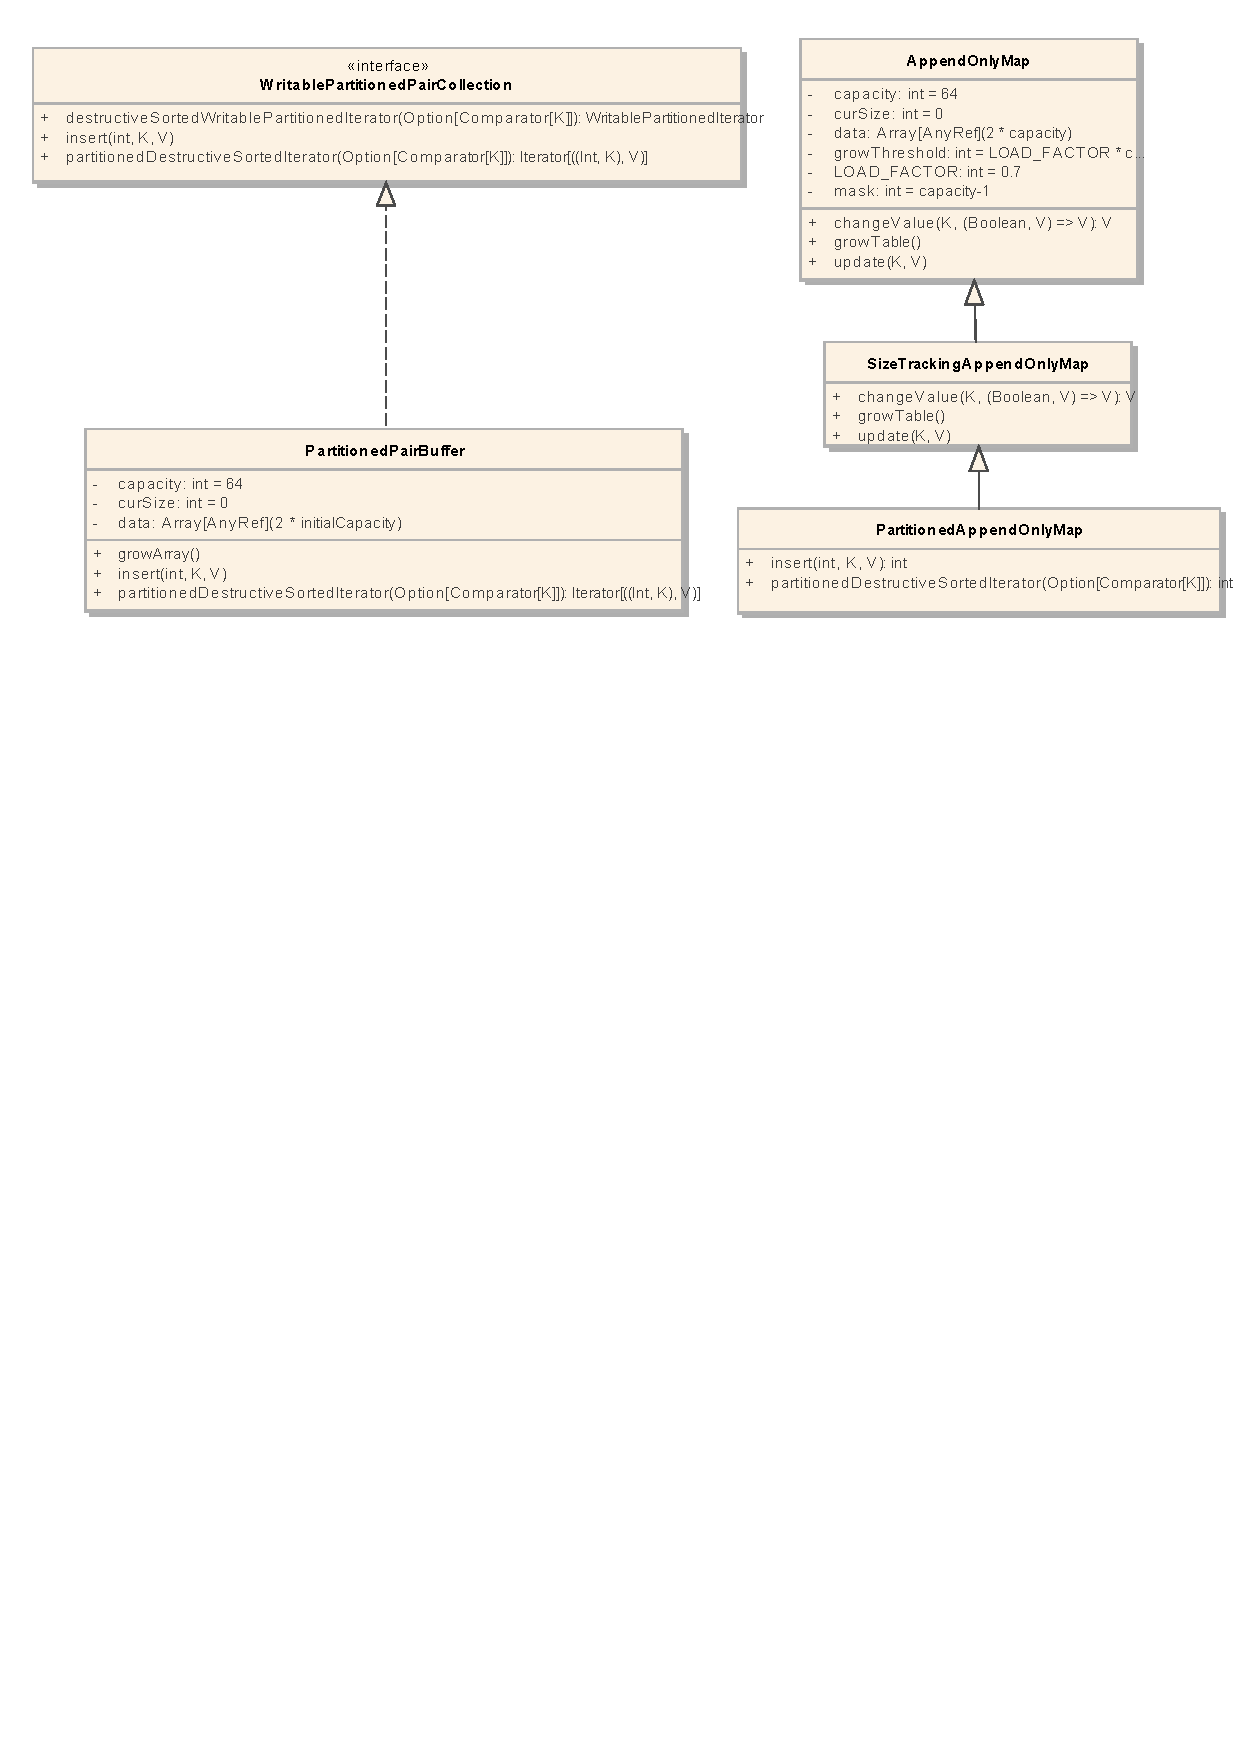
\includegraphics[width=\textwidth]{figures/collection.pdf}
	\caption{Map和Buffer类图}
	\label{fig:mapAndBuffer}
\end{figure}

由上图可以看出reduceBy算法需要map端聚合,map.changeValue调用的是AppendOnlyMap中的changeValue,完成的工作是将记录写到map缓存中,按照reduceByKey算子中定义的合并方法对相同key的value进行处理。如程序\ref{inputPrg:mapChangeValue}所示
\begin{codeInput}{Scala}{缓存并更新value值}{mapChangeValue}
def changeValue(key: K, updateFunc: (Boolean, V) => V): V = {
  assert(!destroyed, destructionMessage)
  val k = key.asInstanceOf[AnyRef]
  //如果传入的key为空值,队列自动增加长度,
  // 这里的设计很巧妙:因为队列自动增加,就肯定会多出一个值,如果你不给它赋值的话,它就为null,
  // 但是这个值又不占队列中具体的位置,只要在最后的时候保留一个没有赋值的位置即可。
  if (k.eq(null)) {
    if (!haveNullValue) {
      incrementSize()
    }
    nullValue = updateFunc(haveNullValue, nullValue)
    haveNullValue = true
    return nullValue
  }
  var pos = rehash(k.hashCode) & mask
  var i = 1
  while (true) {
    //data是一个数组,用来同时存储key和value:key0, value0, key1, value1, key2, value2, etc.
    // 即2 * pos上存储的是key的值,2 * pos + 1上存储的是value的值
    val curKey = data(2 * pos)
    if (k.eq(curKey) || k.equals(curKey)) {
      //如果有相同的值的话,则根据updateFunc更新这个key对应的value
      val newValue = updateFunc(true, data(2 * pos + 1).asInstanceOf[V])
      data(2 * pos + 1) = newValue.asInstanceOf[AnyRef]
      return newValue
    } else if (curKey.eq(null)) {
      //如果key不存在就将该key和对应的value添加到data这个数组中
      val newValue = updateFunc(false, null.asInstanceOf[V])
      data(2 * pos) = k
      data(2 * pos + 1) = newValue.asInstanceOf[AnyRef]
      incrementSize()
      return newValue
    } else {
      //如果pos和其它的key重合,则继续计算其位置
      val delta = i
      pos = (pos + delta) & mask
      i += 1
    }
  }
  null.asInstanceOf[V] // Never reached but needed to keep compiler happy
}
\end{codeInput}
\subsection{shuffle结果本地缓存}
这部分将shuffle结果缓存到本地,并为之生成索引文件,同时返回文件的迭代器。整体过程如程序\ref{inputPrg:cachePartitionFile}所示
\begin{codeInput}{Scala}{完成分区文件和索引文件的本地缓存}{cachePartitionFile}
//打开一个文件
val output = shuffleBlockResolver.getDataFile(dep.shuffleId, mapId)
val tmp = Utils.tempFileWith(output)
//构造blockId
val blockId = ShuffleBlockId(dep.shuffleId, mapId, IndexShuffleBlockResolver.NOOP_REDUCE_ID)
//将数据写入data文件
val partitionLengths = sorter.writePartitionedFile(blockId, tmp)
//将数据写入index文件
shuffleBlockResolver.writeIndexFileAndCommit(dep.shuffleId, mapId, partitionLengths, tmp)
//进行shuffle read时的一些参考信息
mapStatus = MapStatus(blockManager.shuffleServerId, partitionLengths)
\end{codeInput}
\subsubsection{写分区文件}
此步骤负责将缓存在内存map或者buffer中的记录缓存到本地磁盘中,如果之前已经有部分数据溢出到磁盘,会将这些一起进行合并。写分区文件过程如程序\ref{inputPrg:writePartitionFile}所示
\begin{codeInput}{Scala}{生成分区文件并写入数据}{writePartitionFile}
def writePartitionedFile(
blockId: BlockId,
outputFile: File): Array[Long] = {
  val lengths = new Array[Long](numPartitions)
  //首先判断是否有数据已经spill到磁盘了
  if (spills.isEmpty) {
    //当只有内存中有数据时
    val collection = if (aggregator.isDefined) map else buffer
    // 获得迭代器
    val it = collection.destructiveSortedWritablePartitionedIterator(comparator)
    //进行迭代并将数据写到磁盘
    while (it.hasNext) {
      val writer = blockManager.getDiskWriter(blockId, outputFile, serInstance, fileBufferSize,context.taskMetrics.shuffleWriteMetrics.get)
      val partitionId = it.nextPartition()
      while (it.hasNext && it.nextPartition() == partitionId) {
        //把同一个分区的记录写到一块 并返回该blockId中该partitionId的长度
        it.writeNext(writer)
      }
      writer.commitAndClose()
      val segment = writer.fileSegment()
      //最后返回的是每个partition写入数据的长度
      lengths(partitionId) = segment.length
    }
  } else {
    //需要持久化到硬盘中的情况,在调用partitionedIterator方法后,会对应的partition中的已经combine过的数据
    for ((id, elements) <- this.partitionedIterator) {
      if (elements.hasNext) {
        val writer = blockManager.getDiskWriter(blockId, outputFile, serInstance, fileBufferSize,
        context.taskMetrics.shuffleWriteMetrics.get)
        //将partition中的数据写入data文件
        for (elem <- elements) {
          writer.write(elem._1, elem._2)
        }
        writer.commitAndClose()
        val segment = writer.fileSegment()
        //最后返回的是每个partition写入数据的长度
        lengths(id) = segment.length
      }
    }
  }
//更改task测量系统中的参数值
......
lengths
}
\end{codeInput}

上面函数通过判断spills是否为空进行了不同的处理,spills为空时表示记录全部缓存在内存中只需要从内存map或者buffer中取出数据写到本地磁盘即可,spills不为空时,得将已经写到磁盘的和内存中缓存的部分进行合并。接下来分析spills为空时的情况。

程序会获取collection的迭代器,这里会传入比较器,其中destructiveSortedWritablePartitionedIterator是个接口方法,其内部逻辑如程序\ref{inputPrg:destructiveSortedWritablePartitionedIterator}所示
\begin{codeInput}{Scala}{排序分区迭代器}{destructiveSortedWritablePartitionedIterator}
def destructiveSortedWritablePartitionedIterator(keyComparator: Option[Comparator[K]])
: WritablePartitionedIterator = {
  // 这里的partitionedDestructiveSortedIterator会根据是map或者buffer有不同的实现
  val it = partitionedDestructiveSortedIterator(keyComparator)
  // 最后返回的是WritablePartitionedIterator,上面进行写操作的时候就是调用该迭代器中的writeNext方法
  new WritablePartitionedIterator {
    private[this] var cur = if (it.hasNext) it.next() else null	
    def writeNext(writer: DiskBlockObjectWriter): Unit = {
      writer.write(cur._1._2, cur._2)//((partitionId,K),V)
      cur = if (it.hasNext) it.next() else null
    }	
    def hasNext(): Boolean = cur != null	
    def nextPartition(): Int = cur._1._1
  }
}
\end{codeInput}

程序\ref{inputPrg:destructiveSortedWritablePartitionedIterator}中partitionedDestructiveSortedIterator会根据是map或者buffer有不同的实现,由图\ref{fig:mapAndBuffer}可以看出map时其实现在PartitionedAppendOnlyMap,从其实现上可以看出排序逻辑,如程序\ref{inputPrg:PartitionedAppendOnlyMapIter}所示
\begin{codeInput}{Scala}{PartitionedAppendOnlyMap分区排序迭代器实现}{PartitionedAppendOnlyMapIter}
def partitionedDestructiveSortedIterator(keyComparator: Option[Comparator[K]])
: Iterator[((Int, K), V)] = {
  //先它这里会构造一个按partition和key进行比较的比较器,这个比较器先按partition来排序,
  //然后再用key的hashcode进行排序,记住这里spark系统是进行key排序了的,而不是没有排序,只是它这里是按照key的hashcode进行的排序。
  val comparator = keyComparator.map(partitionKeyComparator).getOrElse(partitionComparator)
  //后通过这个比较器再对这个map进行排序
  destructiveSortedIterator(comparator)
}
\end{codeInput}
\subsubsection{写索引文件}
具体的实现就不详细说明了,主要就是根据上一步的到的partition长度的数组将偏移量写入到index文件中。

所以最终每一个task的文件最终产生两个文件,而一个spark程序shuffle产生的数据就取决于并行度或者说reducer的数量,即2*recuder个。

最后就是实例化MapStatus,shuffle read的时候根据MapStatus获取数据。

\subsection{BypassMergeSortShuffleHandle对应BypassMergeSortShuffleWriter}
该writer在进行写记录之前会根据reducer的个数(例如R个)生成R个临时文件,然后将记录写入对应的临时文件中,最后将这些文件进行合并操作并写入到一个文件中,由于直接将记录写入了临时文件,并没有缓存在内存中,所以如果reducer的个数过多的话,就会为每个reducer打开一个临时文件,如果reducer的数量过多的话就会影响性能,所以使用该种方式需要满足一些条件
\begin{enumerate}[\bfseries 1]
	\item 无排序器
	\item 无聚合器
	\item reduce端分区数量<spark.shuffle.sort.bypassMergeThreshold.默认值为200
\end{enumerate}

\subsection{SerializedShuffleHandle对应UnsafeShuffleWriter}

这部分也就是通常所说的Tungsten,在此不做细讲。
\subsection{Shuffle Write流程图}
\begin{figure}[H] 
	\centering
	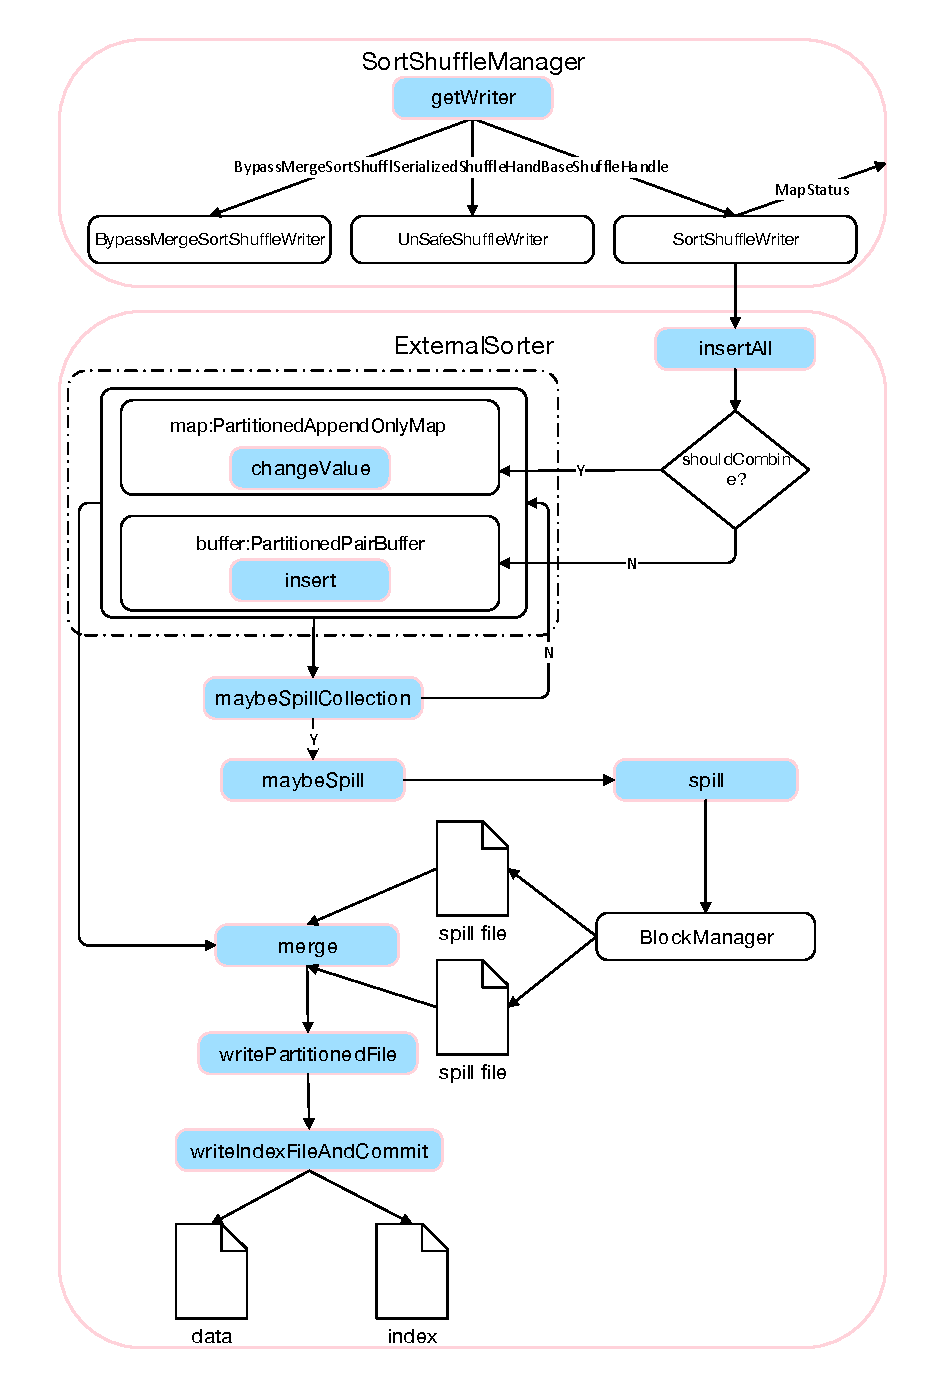
\includegraphics[width=\textwidth,height=0.9\textheight]{figures/sortShuffleWriter.pdf}
	\caption{SortShuffleWriter流程图}
	\label{fig:sortShuffleWriter}
\end{figure}
SortShuffleWriter具体流程如图\ref{fig:sortShuffleWriter}所示
\section{Spark1.6版本Shuffle Read}

在Stage的边界,要计算ShuffledRDD中的数据,必须先把 MapPartitionsRDD 中的数据 fetch 过来。而下边界,要么将文件写入本地文件系统,以供子Stage读取,要么是最后一个Stage,输出结果。

下游Stage的第一个RDD即为ShuffledRDD,其compute方法中会调用shuffleManager.getReader来读取上游的分区,而不管是HashShuffleManager还是SortShuffleManager,其getReader方法内部都是实例化了BlockStoreShuffleReader,而BlockStoreShuffleReader正是实现了ShuffleReader接口。全部 ShuffleMapTasks 执行完再去 fetch。因为 fetch 来的 FileSegments 要先在内存做缓冲,所以一次 fetch 的 FileSegments 总大小不能太大。Spark 规定这个缓冲界限不能超过spark.reducer.maxMbInFlight,这里用sortBuffer表示,默认大小为 48MB。核心的read实现如程序\ref{inputPrg:shuffleReader}所示
\begin{codeInput}{Scala}{Shuffle Read的实现}{shuffleReader}
override def read(): Iterator[Product2[K, C]] = {
val blockFetcherItr = new ShuffleBlockFetcherIterator(context,blockManager.shuffleClient,
blockManager,mapOutputTracker.getMapSizesByExecutorId(handle.shuffleId, startPartition, endPartition),
  SparkEnv.get.conf.getSizeAsMb("spark.reducer.maxSizeInFlight", "48m") * 1024 * 1024)
  // 将上面获取的信息进行压缩处理
  val wrappedStreams = blockFetcherItr.map { case (blockId, inputStream) =>
    blockManager.wrapForCompression(blockId, inputStream)
  }
  //获取序列化器
  val ser = Serializer.getSerializer(dep.serializer)
  ......
  val interruptibleIter = new InterruptibleIterator[(Any, Any)](context, metricIter)	
  val aggregatedIter: Iterator[Product2[K, C]] = if (dep.aggregator.isDefined) {//需要聚合
    if (dep.mapSideCombine) {//需要map端聚合
      val combinedKeyValuesIterator = interruptibleIter.asInstanceOf[Iterator[(K, C)]]
      dep.aggregator.get.combineCombinersByKey(
      combinedKeyValuesIterator, context)
    } else {//只需在reduce端聚合
      val keyValuesIterator = interruptibleIter.asInstanceOf[Iterator[(K, Nothing)]]
      dep.aggregator.get.combineValuesByKey(keyValuesIterator, context)
    }
  } else {//不需要聚合
    interruptibleIter.asInstanceOf[Iterator[Product2[K, C]]]
  }
  dep.keyOrdering match {//判断是否需要排序
    case Some(keyOrd: Ordering[K]) =>
    //对于需要排序的情况使用ExternalSorter进行排序,注意如果spark.shuffle.spill是false,那么数据不会写到磁盘
      val sorter =new ExternalSorter[K, C, C](context, ordering = Some(keyOrd), serializer = Some(ser))
      sorter.insertAll(aggregatedIter)
      ......
      CompletionIterator[Product2[K, C], Iterator[Product2[K, C]]](sorter.iterator, sorter.stop())
    case None =>aggregatedIter
    //无需排序
  }
}
\end{codeInput}

一个 ShuffleMapStage 形成后,会将该 stage 最后一个 final RDD 注册到 MapOutputTrackerMaster.registerShuffle(shuffleId, rdd.partitions.size),这一步很重要,因为 shuffle 过程需要 MapOutputTrackerMaster 来指示 ShuffleMapTask 输出数据的位置”。因此,reducer 在 shuffle 的时候是要去 driver 里面的 MapOutputTrackerMaster 询问ShuffleMapTask输出的数据位置的,它会调用MapOutputTracke.getStatuses来获得数据的meta数据信息,获得meta数据信息后,它会将这些数据存入Seq[(BlockManagerId, Seq[(BlockId, Long)])]中,然后调用ShuffleBlockFetcherIterator最终发起请求。

上述函数会首先实例化ShuffleBlockFetcherIterator,实例化时传入了几个参数,下面几个比较重要
\begin{enumerate}[\bfseries 1]
	\item blockManager.shuffleClient
	\item mapOutputTracker.getMapSizesByExecutorId(handle.shuffleId, startPartition, endPartition)
	\item SparkEnv.get.conf.getSizeAsMb("spark.reducer.maxSizeInFlight", "48m") * 1024 * 1024
\end{enumerate}
\subsection{shuffleClient}
shuffleClient就是用来读取其他executors上的shuffle文件的,其初始化如程序\ref{inputPrg:shuffleClientInitial}所示
\begin{codeInput}{Scala}{创建shuffleClient}{shuffleClientInitial}
private[spark] val shuffleClient = if (externalShuffleServiceEnabled) {
  val transConf = SparkTransportConf.fromSparkConf(conf, "shuffle", numUsableCores)
  new ExternalShuffleClient(transConf, securityManager, securityManager.isAuthenticationEnabled(),
  securityManager.isSaslEncryptionEnabled())
} else {
  blockTransferService
}
\end{codeInput}
由上可知,externalShuffleServiceEnabled默认为false,所以shuffleClient默认为blockTransferService。而blockTransferService在SparkEnv初始化的传入,默认为NettyBlockTransferService,具体细节下一节会讲述。
\subsection{元数据获取}
mapOutputTracker.getMapSizesByExecutorId就是获得该reduce task的数据来源(数据的元数据信息),传入的参数是shuffle的Id和partition的起始位置,返回的是Seq[(BlockManagerId,Seq[(BlockId, Long)])],也就是说数据是来自于哪个节点的哪些block的,并且block的数据大小是多少。如程序\ref{inputPrg:mapOutputTracker}所示
\begin{codeInput}{Scala}{请求元数据}{mapOutputTracker}
def getMapSizesByExecutorId(shuffleId: Int, startPartition: Int, endPartition: Int)
: Seq[(BlockManagerId, Seq[(BlockId, Long)])] = {
  // 获得Map阶段输出的中间计算结果的元数据信息
  val statuses = getStatuses(shuffleId)
  // Synchronize on the returned array because, on the driver, it gets mutated in place
  // 将获得的元数据信息转化成形如Seq[(BlockManagerId, Seq[(BlockId, Long)])]格式的位置信息,用来读取指定的Map阶段产生的数据
  statuses.synchronized {
    return MapOutputTracker.convertMapStatuses(shuffleId, startPartition, endPartition, statuses)
  }
}
\end{codeInput}
最后的getSizeAsMb获取的是一项配置参数,代表一次从Map端获取的最大的数据量。
上述程序中getStatuses用来获取元数据信息,其执行细节如程序\ref{inputPrg:getStatus}所示
\begin{codeInput}{Scala}{获取元数据信息}{getStatus}
private def getStatuses(shuffleId: Int): Array[MapStatus] = {
  // 根据shuffleId获得MapStatus组成的数组:Array[MapStatus]
  val statuses = mapStatuses.get(shuffleId).orNull
  if (statuses == null) {
    //如果没有获取就进行fetch操作
    val startTime = System.currentTimeMillis
    // 用来保存fetch来的MapStatus
    var fetchedStatuses: Array[MapStatus] = null
    fetching.synchronized {
      //其他线程正在请求该shuffleId对应的信息,等待其他线程完成
      while (fetching.contains(shuffleId)) {
        try {
          fetching.wait()
        } catch {
          case e: InterruptedException =>
        }
      }		
      fetchedStatuses = mapStatuses.get(shuffleId).orNull
      if (fetchedStatuses == null) {
        fetching += shuffleId
      }
    }	
    if (fetchedStatuses == null) {
      // 如果得到了fetch的权利就进行抓取
      try {
        // 调用askTracker方法发送消息,消息的格式为GetMapOutputStatuses(shuffleId)
        val fetchedBytes = askTracker[Array[Byte]](GetMapOutputStatuses(shuffleId))
        //MapOutputTrackerMaster返回元数据信息并逆序列化
        fetchedStatuses = MapOutputTracker.deserializeMapStatuses(fetchedBytes)
        // 保存到本地的mapStatuses中
        mapStatuses.put(shuffleId, fetchedStatuses)
      } finally {
        fetching.synchronized {
        fetching -= shuffleId
        fetching.notifyAll()
        }
      }
    }
    if (fetchedStatuses != null) {
      // 最后将抓取到的元数据信息返回
      return fetchedStatuses
    } else {
    } 
  } else {
    // 如果获取到了Array[MapStatus]就直接返回
    return statuses
  }
}
\end{codeInput}
\subsection{根据元数据信息抓取数据}
上节ShuffleBlockFetcherIterator初始化的过程就完成了元数据信息的获取与转换,下面就是根据这些元数据信息抓取对应的数据。ShuffleBlockFetcherIterator实例化的时候会执行一个initialize()方法,用来进行一系列的初始化操作,如程序\ref{inputPrg:ShuffleBlockFetcherIteratorInitialize}所示
\begin{codeInput}{Scala}{ShuffleBlockFetcherIterator初始化}{ShuffleBlockFetcherIteratorInitialize}
private[this] def initialize(): Unit = {
  // 不管最后task是success还是failure,都要进行cleanup操作
  context.addTaskCompletionListener(_ => cleanup())	
  //这里会将本地的数据封装到本地请求块ArrayBuffer[BlockId],返回的为需要远程请求的块,数据结构为ArrayBuffer[FetchRequest]
  val remoteRequests = splitLocalRemoteBlocks()
  // 这里的fetchRequests是一个队列,我们将远程的请求以随机的顺序加入到该队列,然后使用下面的
  // fetchUpToMaxBytes方法取出队列中的远程请求,同时对大小进行限制
  fetchRequests ++= Utils.randomize(remoteRequests)	
  // 从fetchRequests取出远程请求,并使用sendRequest方法发送请求
  fetchUpToMaxBytes()	
  val numFetches = remoteRequests.size - fetchRequests.size
  // 获取本地的Blocks
  fetchLocalBlocks()
}
\end{codeInput}
\subsection{reduce端读取中间计算结果}
ShuffleBlockFetcherIterator会调用splitLocalRemoteBlocks来划分数据的读取方式,主要是本地数据和远程节点数据。这里Spark限制每次最多启动5个线程到最多5个节点上读取数据,同时通过spark.reducer.maxMbInFlight来适应网络带宽。该部分具体情况如程序\ref{inputPrg:spiltLocalRemoteBlocks}所示
\begin{codeInput}{Scala}{reduce读取数据策略划分}{spiltLocalRemoteBlocks}
private[this] def splitLocalRemoteBlocks():ArrayBuffer[FetchRequest]={
  // 为了将大小控制在maxBytesInFlight以下,可以增加并行度,即从1个节点增加到5个
  val targetRequestSize = math.max(maxBytesInFlight / 5, 1L)
  val remoteRequests = new ArrayBuffer[FetchRequest]
  var totalBlocks = 0
  for ((address, blockInfos) <- blocksByAddress) {
    totalBlocks += blockInfos.size
    // 这里就是判断所要获取的是本地的block还是远程的block
    if (address.executorId == blockManager.blockManagerId.executorId) {//本地获取 local
    //Block在本地,需要过滤大小为0的Block
    localBlocks ++= blockInfos.filter(_._2 != 0).map(_._1)
    numBlocksToFetch += localBlocks.size
    } else {//远程获取 remote
      val iterator = blockInfos.iterator
      var curRequestSize = 0L
      var curBlocks = new ArrayBuffer[(BlockId, Long)]
      while (iterator.hasNext) {//blockId是ShuffleBlockId
        val (blockId, size) = iterator.next()
        if (size > 0) {
          curBlocks += ((blockId, size));remoteBlocks += blockId
          numBlocksToFetch += 1;curRequestSize += size
        } else if (size < 0) {
          throw new BlockException(blockId, "block size " + size)
        }
    // 满足大小的限制就构建一个FetchRequest并加入到remoteRequests中
        if (curRequestSize >= targetRequestSize) {
          remoteRequests += new FetchRequest(address, curBlocks)
          curBlocks = new ArrayBuffer[(BlockId, Long)]
          curRequestSize = 0
        }
      }
      if (curBlocks.nonEmpty) {//剩余的请求组成一次Request
        remoteRequests += new FetchRequest(address, curBlocks)
      }
    }
  }
  remoteRequests
}
\end{codeInput}
程序\ref{inputPrg:spiltLocalRemoteBlocks}是用于划分哪些Block从本地获取,哪些需要远程拉取,是获取中间计算结果的关键。程序中下列变量比较重要
\begin{enumerate}[\bfseries 1]
	\item targetRequestSize每个远程请求块的最大尺寸
	\item totalblock统计Block总数
	\item localBlocks:ArrayBuffer[BlockId],缓存本地获取的Block的BlockId序列
	\item remoteBlocks:HashSet[BlockId],缓存远程获取的Block的BlockId序列
	\item curBlocks:ArrayBuffer[(BlockId, Long)],远程获取的累加缓存,用于保证每个远程请求的尺寸不超过targetRequestSize。
	\item  curRequestSize当前curBlocks中的所有Block的大小之和,用于保证每个远程请求尺寸不超过targetRequestSize
	\item remoteRequests:ArrayBuffer[FetchRequest],缓存需要远程请求的FetchRequest对象
	\item numBlocksToFetch,一共要获取的Block数量
	\item maxBytesInFlight,单次航班请求的最大字节数。这批请求的总字节数不能超过maxBytesInFlight,并且每一个请求的字节数不能超过maxBytesInFlight的五分之一。
\end{enumerate}
\subsection{本地数据的获取}
上一小节中已经将本地数据块放入localBlocks,对于本地块中的数据将通过fetchLocalBlocks进行获取。这里就相对简单了,进行迭代,如果获取到就将SuccessFetchResult保存到results中,如果没有就将FailureFetchResult保存到results中具体过程如程序\ref{inputPrg:getLocalBlocks}所示
\begin{codeInput}{Scala}{获取本地块}{getLocalBlocks}
val iter = localBlocks.iterator
while (iter.hasNext) {
  val blockId = iter.next()
  try {
    val buf = blockManager.getBlockData(blockId)
    shuffleMetrics.incLocalBlocksFetched(1)
    shuffleMetrics.incLocalBytesRead(buf.size)
    buf.retain()
    results.put(new SuccessFetchResult(blockId, blockManager.blockManagerId, 0, buf))
  } catch {
  }
}
\end{codeInput}
这里调用了BlockManager.getBlockData获取数据,对于shuffle数据其会调用对应的ShuffleManager.shuffleBlockResolver.getBlockData方法获取数据,其实现如程序\ref{inputPrg:sortShuffleGetBlockData}所示
\begin{codeInput}{Scala}{SortShuffleManager读取shuffle数据实现}{sortShuffleGetBlockData}
//根据ShuffleId和MapId获得索引文件
val indexFile = getIndexFile(blockId.shuffleId, blockId.mapId)
val in = new DataInputStream(new FileInputStream(indexFile))
try {
  ByteStreams.skipFully(in,blockId.reduceId*8)//本次Block的数据区
  val offset = in.readLong()//开始
  val nextOffset = in.readLong()//结束
  new FileSegmentManagedBuffer(transportConf,getDataFile(
  blockId.shuffleId, blockId.mapId),offset,nextOffset - offset)
} 
\end{codeInput}

可以看出它是根据索引文件来获得数据块在数据文件中的具体位置信息的。
\subsection{远程数据的获取}
splitLocalRemoteBlocks返回值为远程数据块,ShuffleBlockFetcherIterator.fetchUpToMaxBytes来发送远程获取请求。通过sendRequest发送读取Block的请求,其中包含中两个回调函数,分别对应着请求成功和请求失败,具体如程序\ref{inputPrg:fetchRemoteBlocks}所示
\begin{codeInput}{Scala}{向远程节点发送读取Block请求}{fetchRemoteBlocks}
private[this] def sendRequest(req: FetchRequest) {
  req.blocks.size, Utils.bytesToString(req.size), req.address.hostPort))
  bytesInFlight += req.size
  //首先获得要fetch的blocks的信息
  val sizeMap = req.blocks.map { case (blockId, size) => (blockId.toString, size) }.toMap
  val blockIds = req.blocks.map(_._1.toString)	
  val address = req.address
  // 然后通过shuffleClient的fetchBlocks方法来获取对应远程节点上的数据
  // 默认是通过NettyBlockTransferService的fetchBlocks方法实现的
  shuffleClient.fetchBlocks(address.host, address.port, address.executorId, blockIds.toArray,
    new BlockFetchingListener {
      // 最后,不管成功还是失败,都将结果保存在results中
      override def onBlockFetchSuccess(blockId: String, buf: ManagedBuffer): Unit = {//请求成功
        if (!isZombie) {
          buf.retain()
          results.put(new SuccessFetchResult(BlockId(blockId), address, sizeMap(blockId), buf))
          shuffleMetrics.incRemoteBytesRead(buf.size)
          shuffleMetrics.incRemoteBlocksFetched(1)
        }
      }	
      override def onBlockFetchFailure(blockId: String, e: Throwable): Unit = {
        results.put(new FailureFetchResult(BlockId(blockId), address, e))
      }
   })
}
\end{codeInput}

请求的结果最终保存在了results中,成功的就是SuccessFetchResult,失败的就是FailureFetchResult

程序中的shuffleClient就是blockTransferService,如程序\ref{inputPrg:shuffleClient}所示
\begin{codeInput}{Scala}{BlockManager获取shuffleClient}{shuffleClient}
val externalShuffleServiceEnabled = conf.getBoolean("spark.shuffle.service.enabled", false)
//externalShuffleServiceEnabled默认为false
private[spark] val shuffleClient = if (externalShuffleServiceEnabled) {
  val transConf = SparkTransportConf.fromSparkConf(conf, "shuffle", numUsableCores)
  new ExternalShuffleClient(transConf, securityManager, securityManager.isAuthenticationEnabled(),
  securityManager.isSaslEncryptionEnabled())
} else {
  blockTransferService
}
//此部分在SparkEnv里定义,直接通过netty的方式
val blockTransferService = new NettyBlockTransferService(conf, securityManager, numUsableCores)
\end{codeInput}
\subsection{BlockStoreShuffleReader.read方法}
上面的步骤获取了数据,接下来的是对这些数据进行处理。具体细节如程序\ref{inputPrg:shuffleReader}所示。程序\ref{inputPrg:shuffleReader}中aggregator和keyOrdering的部分在分析Shuffle Write的时候已经分析过了,这里就不再赘述。
\subsection{Shuffle Read流程图}
整个shuffle read的执行过程如图\ref{fig:shuffleread}所示
\begin{figure}[H] 
	\centering
	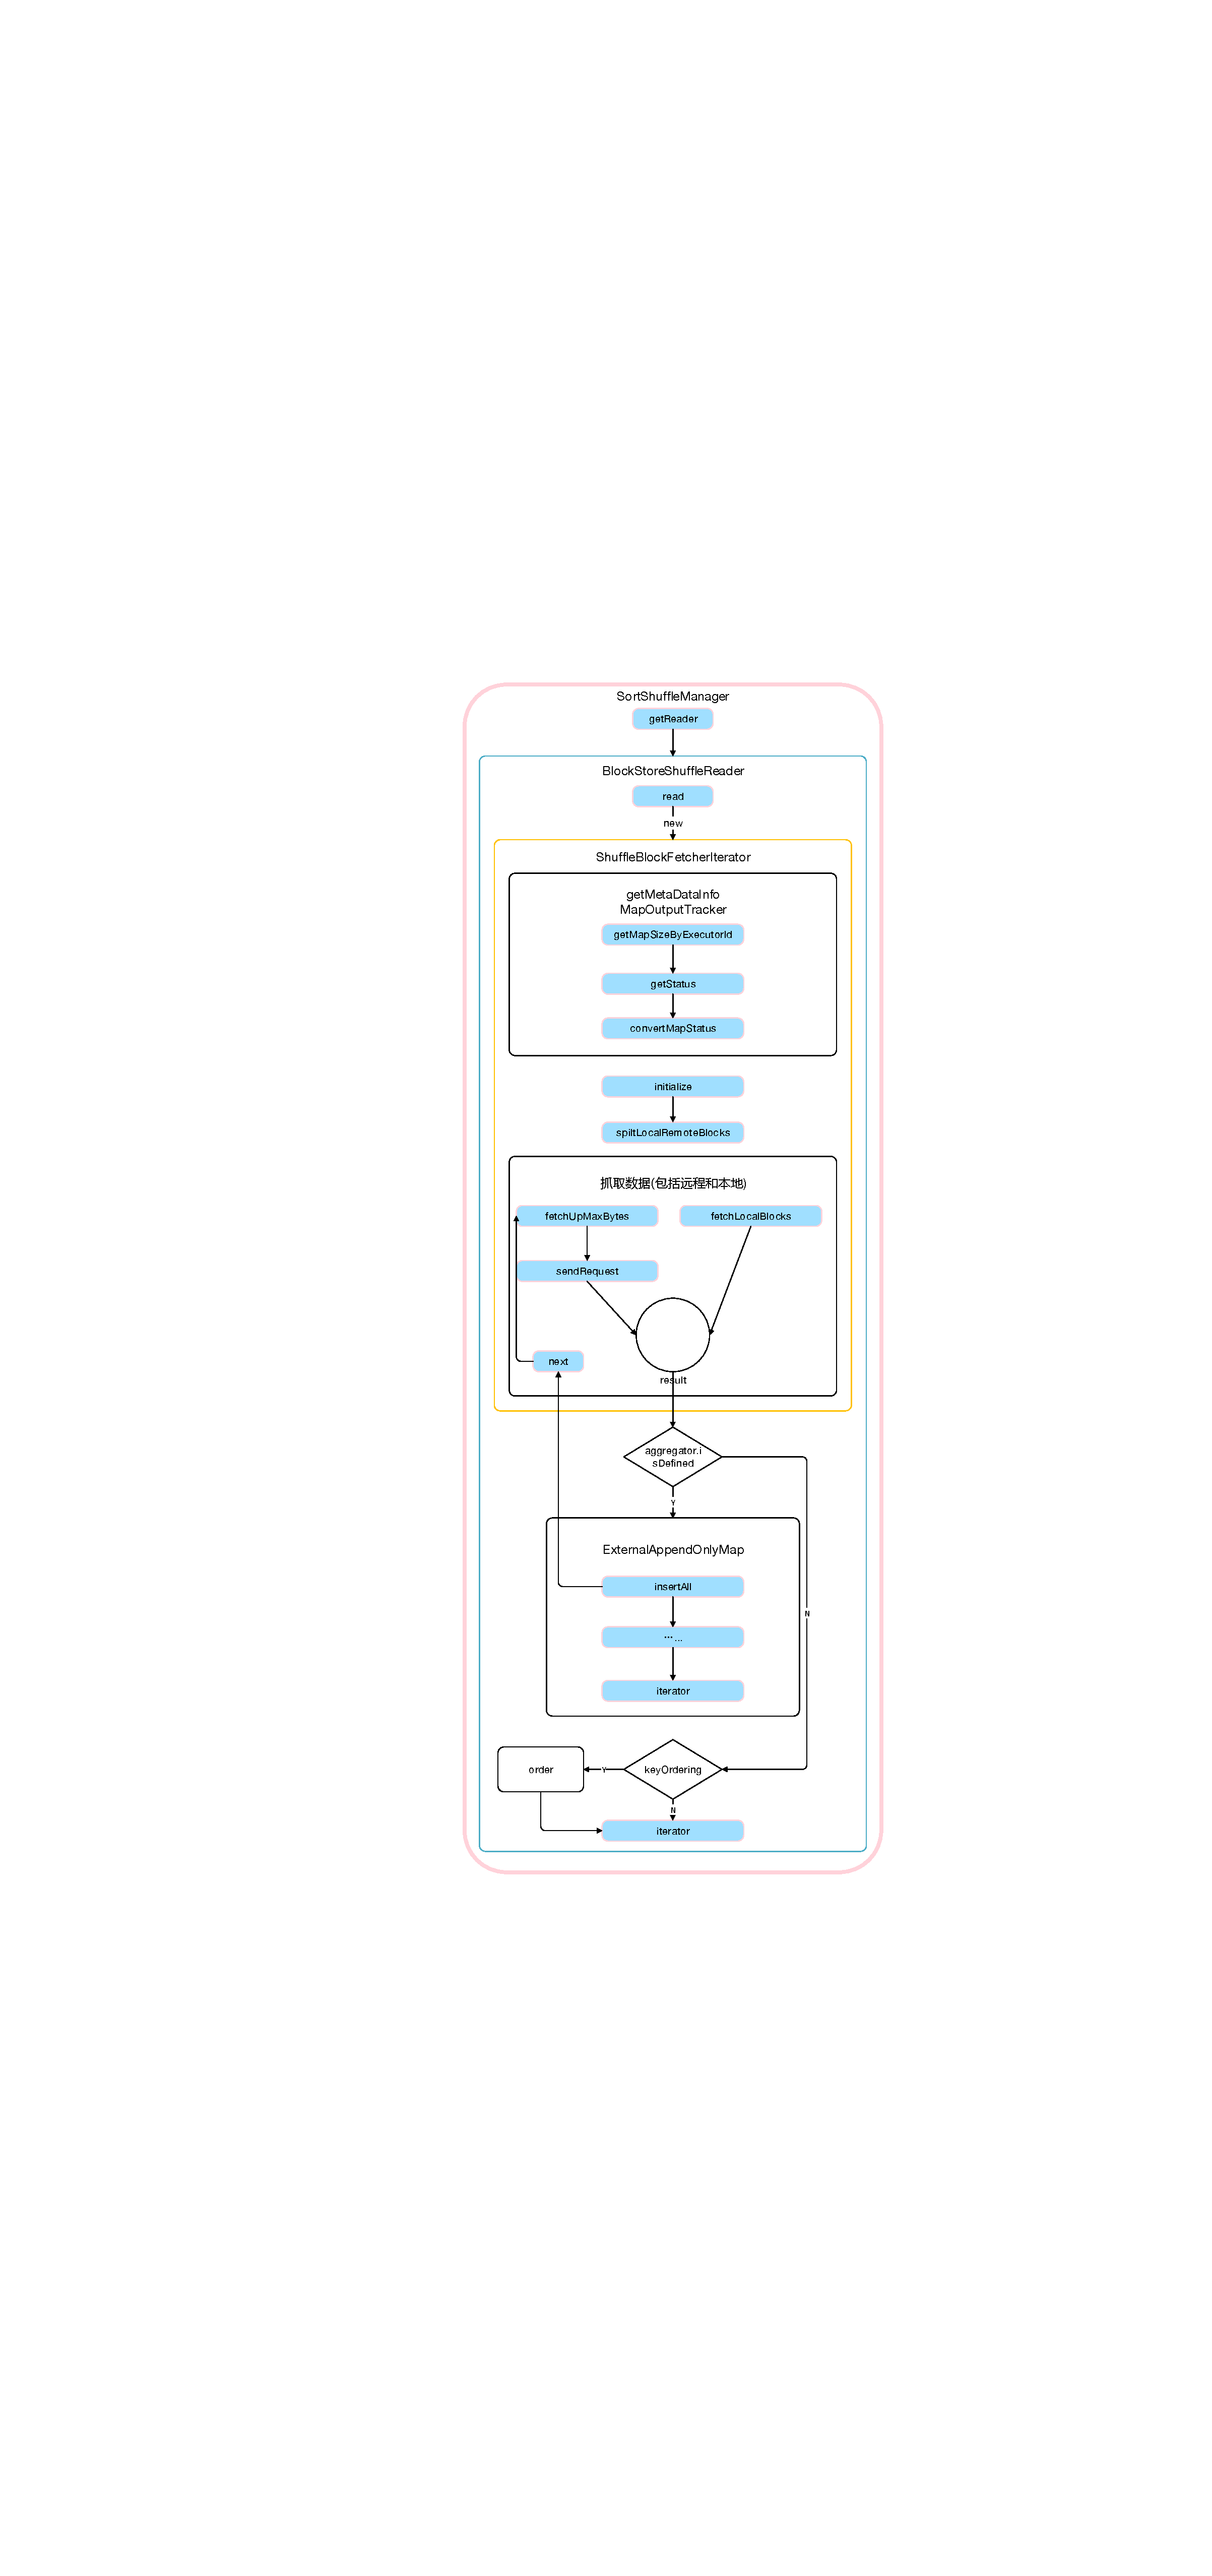
\includegraphics[width=0.85\textwidth,height=0.97\textheight]{figures/sortShuffleReadDia.pdf}
	\caption{shuffleread详细实现}
	\label{fig:shuffleread}
\end{figure}